%-------------------------------------------------------------------------------
% TEYSSIER Maxime
% IUT Béziers - LP Réseaux et Télécommunications - Promotion: 2018/2019
% Stage IUT de Béziers
% Intitulé: WalkersVision
% Tuteur: DRUON Sebastien
%-------------------------------------------------------------------------------

%-------------------------------------------------------------------------------
% Titre du fichier
%-------------------------------------------------------------------------------
\title{Rapport_WalkersVision}

%-------------------------------------------------------------------------------
% Fonctionnalités
%-------------------------------------------------------------------------------
\documentclass[12pt, french]{report}
\usepackage[a4paper]{geometry}
\usepackage[myheadings]{fullpage}
\usepackage[french]{babel}
\usepackage[T1]{fontenc}
\usepackage[utf8]{inputenc}
\usepackage{sectsty}
\usepackage[font=small, labelfont=bf]{caption}
\usepackage{fourier}
\usepackage[protrusion=true, expansion=true]{microtype}
\usepackage{fancyhdr}
\usepackage{lastpage}
\usepackage{graphicx, wrapfig, subcaption, setspace, booktabs}
\usepackage{titletoc}
\usepackage{hyperref}
\usepackage{tikz}
\usepackage{multicol}
\usepackage{xcolor}
\usepackage{color}
\usepackage{url}
\usepackage{minted}
\onehalfspacing
\setcounter{tocdepth}{5}
\setcounter{secnumdepth}{5}
\renewcommand{\thesection}{\arabic{section}}
\newcommand{\HRule}[1]{\rule{\linewidth}{#1}}
\definecolor{LightGray}{gray}{0.7}


\usepackage{tikz}
\usepackage{amsmath}

%-------------------------------------------------------------------------------
%Début du document
%-------------------------------------------------------------------------------
\begin{document}

%-------------------------------------------------------------------------------
% En-tête & pied de page
%-------------------------------------------------------------------------------
\pagestyle{fancy}
\fancyhf{}
\setlength\headheight{15pt}
\fancyhead[L]{Maxime TEYSSIER}
\fancyhead[R]{IUT de Béziers}
\fancyfoot[R]{Page \thepage\ sur \pageref{LastPage}}

%-------------------------------------------------------------------------------
% Page de garde
%-------------------------------------------------------------------------------

\title{
\includegraphics[width=0.56\textwidth]{Images/IUT-Beziers.png}\\
		\normalsize\textsc{}
		\HRule{2pt} \\
        \LARGE \textbf{\uppercase{Rapport de stage\\Comptage et statistiques de passants sur une place publique par analyse}}
		\HRule{2pt} 
		\normalsize 04 Juin 2019 - 27 Août 2019 \vspace*{3\baselineskip}
        }
\author{Stagiaire: Maxime TEYSSIER\\Tuteur: Sébastien DRUON\\ 
        
\includegraphics[width=0.25\textwidth]{Images/UM.png}
        \date{}\\
        }
\maketitle
\clearpage
\newpage
%%%%%%%%%%%%%%%%%%%%%%%%%%%%%%%%%%%%%%%%%%%%%%%%%%%%%%%%%%%%%%%%%%%%%%%%%%%%%%%
%%%%%%%%%%%%%%%%%%%%% Page blanche sans mise en page %%%%%%%%%%%%%%%%%%%%%%%%%%
%%%%%%%%%%%%%%%%%%%%%%%%%%%%%%%%%%%%%%%%%%%%%%%%%%%%%%%%%%%%%%%%%%%%%%%%%%%%%%%
\strut									      %
\thispagestyle{empty}							      %
\newpage							              %
%%%%%%%%%%%%%%%%%%%%%%%%%%%%%%%%%%%%%%%%%%%%%%%%%%%%%%%%%%%%%%%%%%%%%%%%%%%%%%%

%----------------Remerciements--------------------------------------------------
\section*{Remerciements}
J'adresse mes remerciements aux personnes qui m'ont permis à réaliser ce stage au sein de l'IUT de Béziers.

\bigskip

En premier lieu, M. Sébastien DRUON,\\
Je souhaite remercier\\
Je tiens à remercier aussi \\

\newpage

%-------------------------------------------------------------------------------
%-------------------------------------------------------------------------------
% Sommaire								       
%-------------------------------------------------------------------------------

\tableofcontents
\clearpage 

%-------------------------------------------------------------------------------
% Début des écrits
%-------------------------------------------------------------------------------

%%%%%%%%%%%%%%%%%%%%%%%%%%%%%
\startcontents[mainsections]%
%%%%%%%%%%%%%%%%%%%%%%%%%%%%%

\section{Introduction}

    % Mise en explication du sujet
    % Identification du besoin
    % Modelisation du terrain 


% A la recherche d'une intro
    % 1/
    %"Les recensements de population constituent la source principale des études sociodémographiques portant sur le local, et en particulier sur le niveau infra communal, celui des quartiers. Ils permettent des descriptions des caractéristiques du peuplement des quartiers sous l’aspect structurel en appréciant les écarts avec leur environnement proche, par exemple celui de la commune ou de l’unité urbaine à laquelle ils appartiennent." \url{www.cairn.info/revue-francaise-des-affaires-sociales-2001-3-page-39.htm}

    % 2/
        Le domaine de vision par ordinateur, poussé par les progrès scientifiques et technologiques récents, s’oriente vers l’analyse en temps réel des scènes comportant des sujets humains. (Source: \url{https://tel.archives-ouvertes.fr/tel-00004804/document} ) %- titre / auteur: Vision par ordinateur pour l’interaction homme-machine fortement couplée - De François Bérard - Thèse) \\
       
       \textbf{FAIRE L'INTRODUCTION !}

\newpage
\section*{Présentation}
\subsection*{L'établissement}

L'Institut Universitaire de Technologie de Béziers propose des formations universitaires alliant théorie et pratique qui répondent aux attentes des entreprises en termes de formation technologique. \\

Depuis 2011, l’IUT de Béziers s’est installé dans ses nouveaux locaux, place du 14 juillet. Proche du centre-ville, il s’inscrit parfaitement dans la vie de ce quartier qui accueille déjà la Médiathèque André Malraux, l’antenne Du Guesclin de l’Université Paul-Valéry et le Centre interrégional de développement de l’occitan.\\

\textbf{Directeur}: Philippe Pujas\\

\textbf{Directrice administrative}: Annie Molès\\
\bigskip

\textbf{Quelques chiffres}\\
\begin{itemize}
        \item 510 étudiants en formation continue, 49 en apprentissage
        \item 3 départements d'enseignement: Réseaux et Télécommunications, Métiers du Multimédia et de l'Internet, Techniques de commercialisation
        \item Plus de 100 partenaires entreprises\\
\end{itemize} 


\textbf{Contact}:\\ 3, Place du 14 juillet,\\ BP 50438,\\ 34505 Béziers cedex\\ Tél.: +33(0)4 67 11 60 00


\subsection*{Les missions}
\subsection*{Horaires}
Dans le cadre du stage, je dois faire 35h par semaine. Les horaires étaient données :
9h00 - 12h00, 13h00 - 17h00.

\begin{center}
        \begin{tabular}{|l|l|l|l|l|c|r|}
                \hline
                Lundi & Mardi & Mercredi & Jeudi & Vendredi \\
                \hline
                8h00 - 12h00 & 8h00 - 12h00 & 8h00 - 12h00 & 8h00 - 12h00 & 8h00 - 12h00 \\
                13h00 - 17h00 & 13h00 - 17h00 & 13h00 - 17h00 & 13h00 - 17h00 & 13h00 - 17h00 \\ 
                \hline
        \end{tabular}
\end{center}
\newpage

\section{Les missions}


Le stage a pour but d'être utile pour la ville de Béziers. La mission est une solution qui créer des statistiques de passants sur une place public. \\

La mission est, dans un premier temps, de connaître le nombre de passants sur la place en temps réel. Les données traitées seront envoyés vers un serveur via TCP/IP ou LoRa. Seul des données transiterons. Aucune image sera transmise.\\ 

Dans un second temps, nous essayerons de remonter l'endroit ou ce trouve les passants sur la place et connaitre leur typologie (adulte/enfant).\\

De plus, un dimensionnement de camera est à réaliser.
\newpage
%%%%%%%%%%%%%%%%%%%%% Page blanche avec mise en page %%%%%%%%%%%%%%%%%%%%%%%%%%
\strut									      %
\newpage							              %
%%%%%%%%%%%%%%%%%%%%%%%%%%%%%%%%%%%%%%%%%%%%%%%%%%%%%%%%%%%%%%%%%%%%%%%%%%%%%%%
\newpage

\section{Traitement d'image}
Avant de traiter une image, qu'est ce qu'une image? Une image est une matrice de valeurs. Les valeurs diffèrent de la propriété de l'image. Lorsque je vais prendre une image elle aura des valeurs qui définit les couleurs sur un espace de couleur BGR (Blue - Green - Red).

        \subsection{Ouvrir et afficher une image}
                Une image peut être enregistrer sur un disque sous format .jpg, .png... Dans ce cas là, une fonction nous permettra de charger l'image. Pour cela nous utiliserons "imread()". Cela dit, via une webcam nous pouvons prendre une photo et la charger. Pour cela, nous utiliserons la fonction "VideoCapture". Deux choix sont possible: utiliser une image déjà créer ou prendre une photo.


                \subsubsection{"imread"}
                Le fonction \textit{imread()} va nous servir pour traiter dans un premier temps une image enregistré sur le disque.
                L'image en question est Lena ou Lenna.
                Cette photo est un standart dans le test d'image pour deux raison selon David C. Munson, éditeur en chef lors des discussions de l'IEEE sur le traitement d'image de janvier 1996: 
                "Tout d'abord, cette image contient un mélange intéressant de détails, de régions uniformes, et de textures, ce qui permet de bien tester les différents algorithmes de traitement d'image. C'est une bonne image de test ! Ensuite, « Lenna » est l'image d'une femme attirante. Ce n'est pas une surprise que la communauté de la recherche dans le traitement d'image (principalement masculine) gravite autour d'une image qu'elle trouve attirante." 
                \begin{center}
                        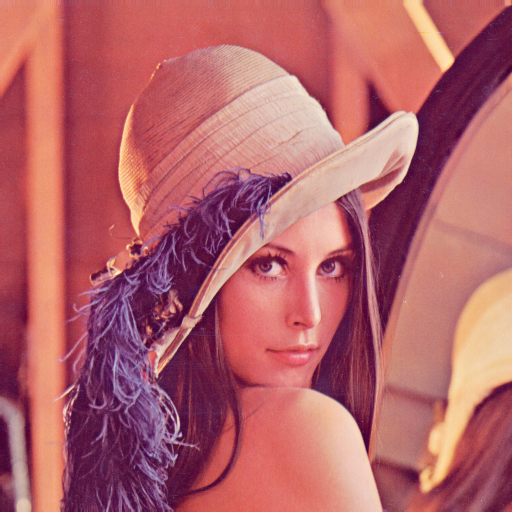
\includegraphics[width=0.4\textwidth]{Images/Lenna.png}\\
                        \textit{Photo 1 - Lenna}\\
                \end{center}

                \begin{minted}[
                    baselinestretch=1.4,
                    bgcolor=LightGray,
                    fontsize=\footnotesize]
                    {c++}
#include <opencv2/opencv.hpp>
using namespace cv;
int main(int argc, char** argv ){
    if ( argc != 2 ){ //Si le nombre d argument dépasse 2 (le prog+le nom de l image)
        printf("usage: programme <Image_Path>\n");// Affichage message
        return -1; // ERROR
    }
    Mat image; // Stocke les donnees de l image dans la tableau de classe Mat
    image = imread( argv[1], 1 ); // Charge la matrice que l'image represente
    if ( !image.data ){// Si la matrice n'a pas de valeur
        printf("No image data \n");
        return -1; // ERREUR
    }
    namedWindow(argv[1], WINDOW_AUTOSIZE ); // On nom une fenêtre 
    imshow(argv[1], image); //Affiche l'image dans la fenêtre 
    waitKey(0); // Attend une action via une touche pour quitter
    return 0;
}
                \end{minted}
                \begin{center}
                    \textit{Programme 1 - Chargement d'une image et affichage}\\
                \end{center}
                
                Résultat après compilation et exécution: 
                \begin{center}
                        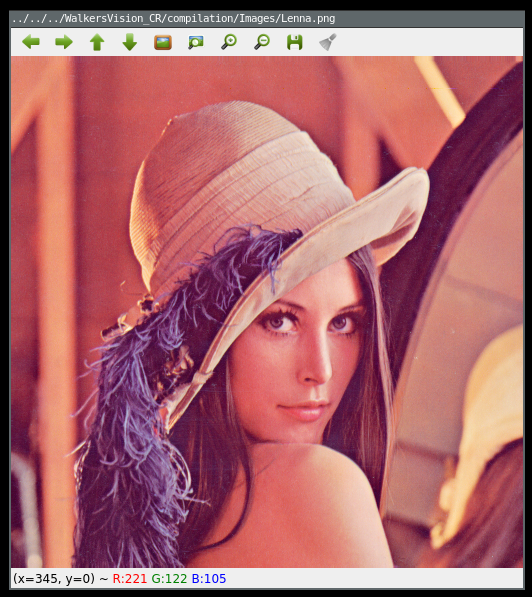
\includegraphics[width=0.5\textwidth]{Images/PrintImageSimple.png}\\
                        \textit{Résultat 1 - Affichage d'une image chargé}
                \end{center}

                \subsubsection{"VideoCapture"}
                La fonction \textit{VideoCapture} nous permet de prendre une instantanée via une caméra.
                \begin{minted}[
                    baselinestretch=1.4,
                    bgcolor=LightGray,
                    fontsize=\footnotesize]
                    {c++}

#include "opencv2/opencv.hpp"
using namespace cv;
int main (int argc, char **argv){
  VideoCapture camera(atoi (argv[1])); Ouvre la caméra demandé en argument
  if (!camera.isOpened ()){return -1;}
      Mat image;
      camera >> image;	//Récupère l'image depuis la caméra
      imshow ("Webcam", image); // Affiche l'image
      waitKey (0)
  return 0;
}
               \end{minted}
               \begin{center}
                   \textit{Prise d'instantanée depuis caméra et affichage}
               \end{center}

                Résultat après compilation et exécution: 
               \begin{center}
                   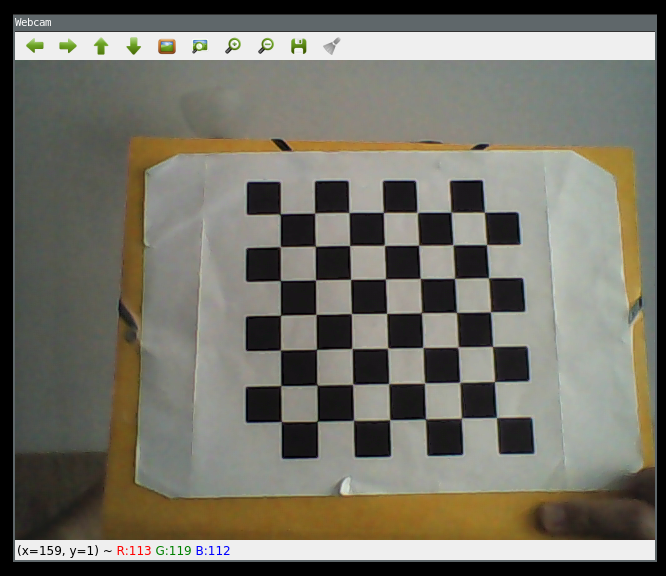
\includegraphics[width=0.5\textwidth]{Images/PhotoWebcam.png}\\
                   \textit{Résultat 2 - Prise d'instantanée et affichage}
               \end{center} 
                

        \subsection{Changement d'espace de couleur}
            Le changement d'espace de couleur permet de voir différemment la même image et ainsi la traiter avec plus d'efficacité. Voici deux espace de couleur différente à BGR, les différentes luminances de gris et les teintes-saturation-valeur (HSV).
            Pour effectuer ce changement, l'utilisation de la fonction \textit{cvtColor()} sera utile.
                \subsubsection{BGR2GRAY}
                Voici un code qui permet de passer de l'espace de couleur BGR en celui de gris: 
                
                \begin{minted}[
                    baselinestretch=1.4,
                    bgcolor=lightgray,
                    fontsize=\footnotesize]
                    {c++}
#include <opencv2/opencv.hpp>
using namespace cv;
int main(int argc, char ** argv){
        char * imageName = argv[1]; // on recupère le chemin où est l'image
        Mat image;
        image =imread(imageName);
        if(argc!=2 || !image.data){
                printf("ERROR");
                return -1;
        }
        Mat gray_image;
        // cvtColor(source, destination, traduction d'espace de couleur)
        cvtColor(image, gray_image, COLOR_BGR2GRAY); 
        imshow(imageName, image);
        imshow("Gray image", gray_image);
        waitKey(0);
        return 0;
}
                \end{minted}
                
                \begin{center}
                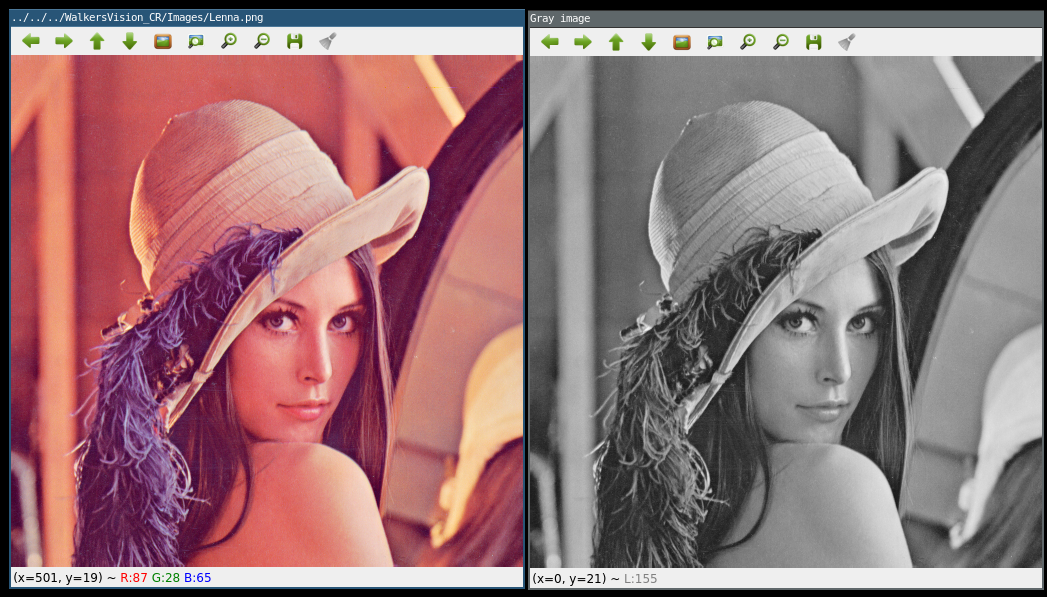
\includegraphics[width=0.8\textwidth]{Images/ImgBGR2GRAY.png}\\
                \textit{Résultat 3 - Affichage image normal et teinte de gris}
                \end{center}


                \subsubsection{BGR2HSV}
                Pour notre mission de compter des passants, nous avons besoin de reconnaître un humain d'un arbre ou bâtiment. Dans l'espace de couleur HSV (Hue, Saturation, Value) à la différence d'autres espaces de couleurs, tout les humains ont la même teinte (Hue).
                Pour changer l'espace BGR en HSV, le code est le quasi le même que précédent sauf un paramètre dans \textit{cvtColor}:\\
                
                \begin{minted}[
                 baselinestretch=1.4,
                bgcolor=lightgray,
                fontsize=\footnotesize]
                {c++}
#include <opencv2/opencv.hpp>
using namespace cv;
int main(int argc, char ** argv){
        char * imageName = argv[1]; 
        Mat image;
        image =imread(imageName);
        if(argc!=2 || !image.data){ printf("ERROR"); return -1;}
        Mat hsv_image;
        cvtColor(image, hsv_image, COLOR_BGR2HSV); 
        imshow(imageName, image);
        imshow("Lena HSV", hsv_image);
        waitKey(0);
        return 0;
}
                \end{minted}

                \begin{center}
                 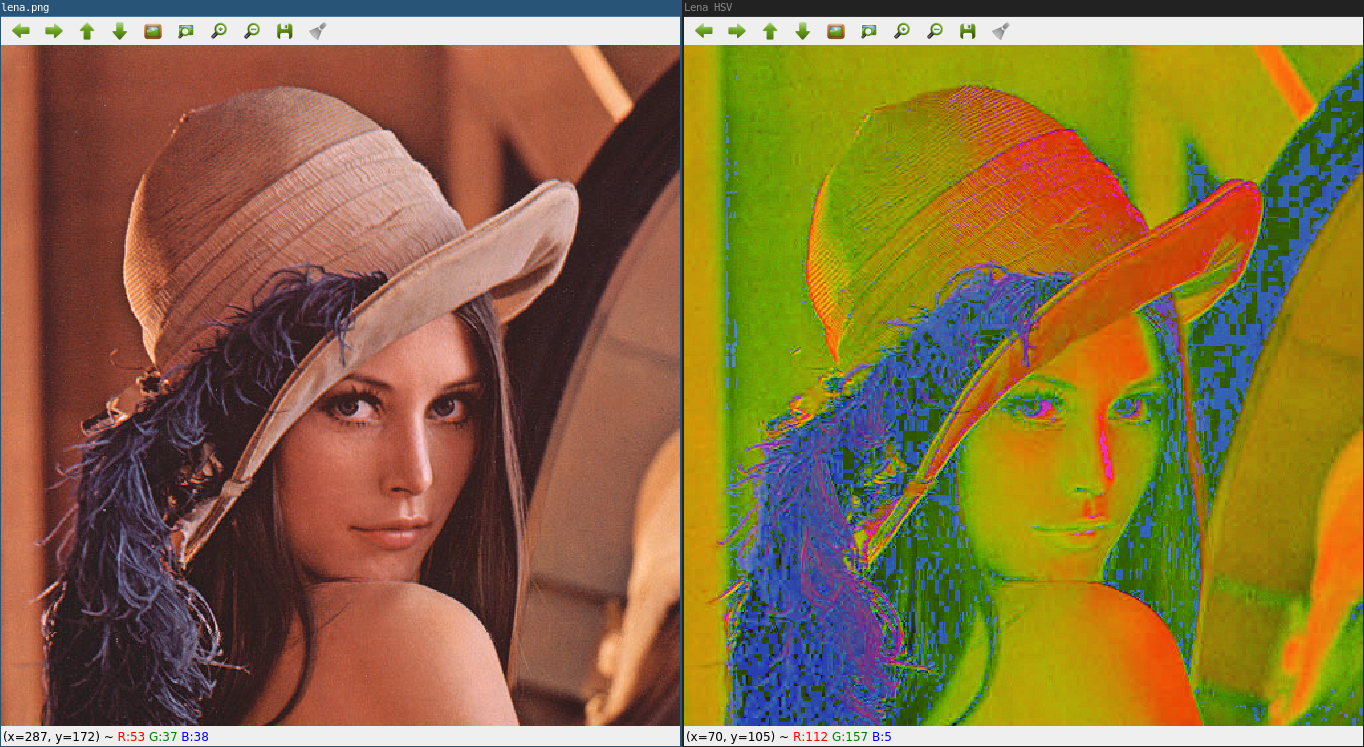
\includegraphics[width=0.8\textwidth]{Images/BGR2HSV.png}\\
                 \textit{Traduction d'espace BGR en HSV}
                \end{center}
                
                
        \subsection{Capturer la peau humaine}
        Pour capturer la peau humaine sur une image, le traitement de l'image par l'espace de couleur HSV est possible. Pour cela, il faut définir une plage de couleur (dans l'espace HSV) à garder. Ainsi, l'extraction affichera la peau humaine.\
        
        \begin{minted}[
        baselinestretch=1.4,
        bgcolor=lightgray,
        fontsize=\footnotesize]
        {c++}
#include <opencv2/opencv.hpp>
using namespace cv;
using namespace std;
int main (int argc, char *argv[]){
    Mat frame, frame_HSV, frame_threshold, PH;
    frame =imread(argv[1], IMREAD_COLOR);
    PH = frame.clone ();
    cvtColor (frame, frame_HSV, COLOR_BGR2HSV, 0);
    inRange (frame_HSV, Scalar (1, 3, 150), Scalar (9, 147, 240),
	       frame_threshold);
    for (int i = 0; i < PH.rows; i++){
	    for (int j = 0; j < PH.cols; j++){
	        if (frame_threshold.at < unsigned char >(Point (j, i)) != 255){
		        PH.at < Vec3b > (Point (j, i)) = Vec3b (0, 0, 0);
		    }
	    }
	}
    imshow ("Image Traite", PH);
    imshow ("Image", frame);
    waitKey(0); 
    return 0;
}
    \end{minted}
                
    \begin{center}
        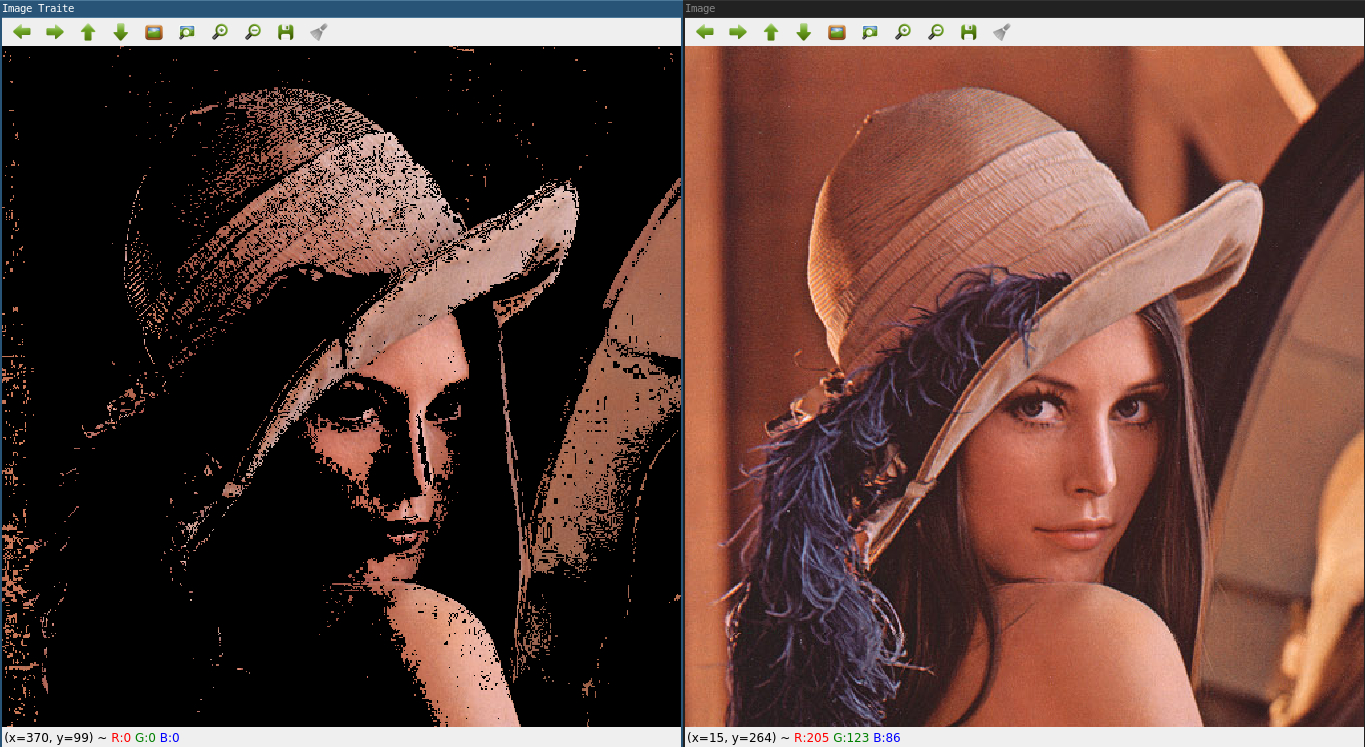
\includegraphics[width=0.8\textwidth]{Images/CPH.png}\\
        \textit{Capture de la peau humaine avec des parasites}
    \end{center}

    Le traitement ne permet pas d'avoir un résultat parfait. Pour améliorer le filtre, l'utilisation de dilatation et érosion de pixel.\\
    
    \subsection{Suppression de fond}
    \subsubsection{pMOG2}
    
    Sur l'étape précédente, le résultat nous affiche le fond d'une image alors que le résultat devrait être juste la peau humaine. Cela dit, si la couleur est dans la même tranche de valeur accepté que celle demandé l'objet va apparaître sur l'image. 
    Pour y remédier, la suppression de fond est nécessaire. Pour la réalisation, l'utilisation d'une vidéo est exigé car le programme ci-dessous, permet de supprimer tout ce qui ne bouge pas, soit le fond. 
    
    \begin{minted}[
    baselinestretch=1.4,
    bgcolor=lightgray,
    fontsize=\footnotesize]
{c++}
#include "opencv2/imgcodecs.hpp"
#include "opencv2/imgproc.hpp"
#include "opencv2/videoio.hpp"
#include <opencv2/highgui.hpp>
#include <opencv2/video.hpp>
#include <stdio.h>
#include <iostream>
#include <sstream>

using namespace cv;
using namespace std;

Mat frame,fgMaskMOG2; 
Ptr<BackgroundSubtractor> pMOG2; 
int keyboard; 
void processWcam(char* videoFilename){
    VideoCapture capture(atoi(videoFilename));

    if(!capture.isOpened()){exit(EXIT_FAILURE);}
    
    while( (char)keyboard != 'q'  && (char)keyboard != 27 ){
        if(!capture.read(frame)) {exit(EXIT_FAILURE);}
        GaussianBlur(frame,frame,Size(5,5),0,0);
        GaussianBlur(frame,frame,Size(5,5),0,0);
        pMOG2->apply(frame, fgMaskMOG2);
        stringstream ss;

        imshow("Frame", frame);
        imshow("FG Mask MOG 2", fgMaskMOG2);
        keyboard = waitKey(30);
    }
    capture.release();
}
int main(int argc, char* argv[]){
    while(true){
            pMOG2 = createBackgroundSubtractorMOG2(); 
            processWcam(argv[1]);
            destroyAllWindows();
            return EXIT_SUCCESS;
        }
}

\end{minted}
    
    \begin{center}
        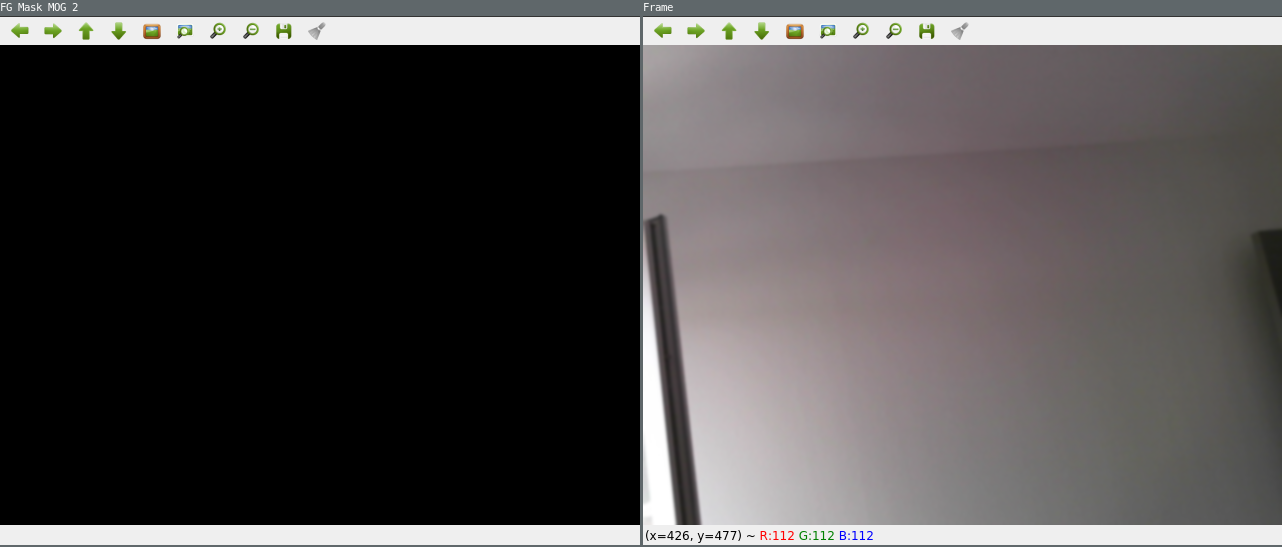
\includegraphics[width=0.8\textwidth]{Images/BGSub/BGSub0.png}\\
        \textit{Suppression du fond lors d'aucun mouvement}
    \end{center}
    
    \begin{center}
        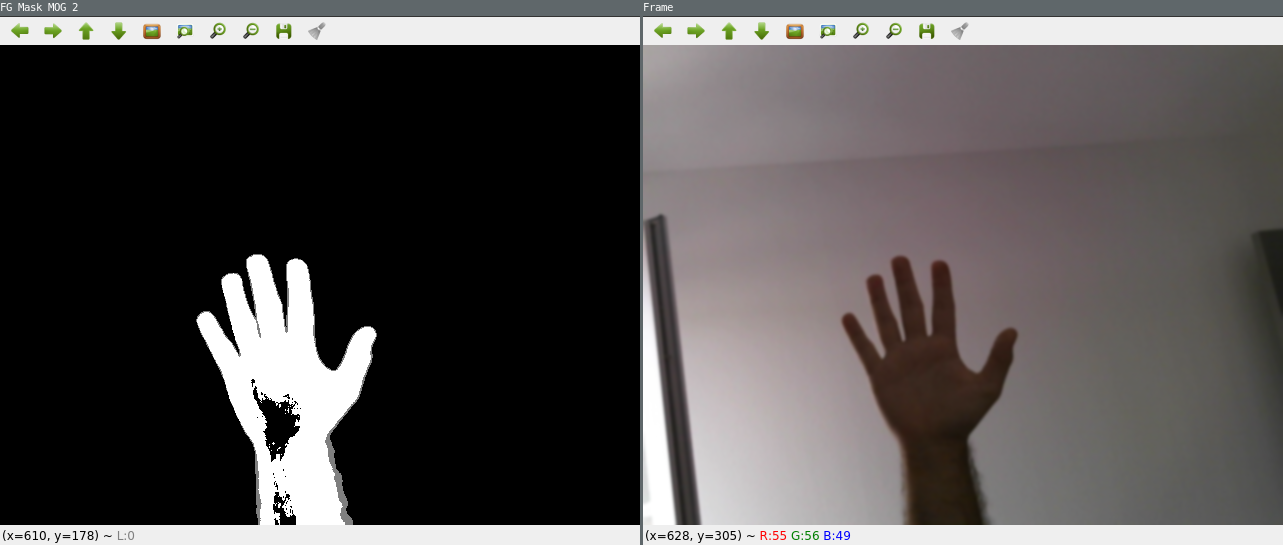
\includegraphics[width=0.8\textwidth]{Images/BGSub/BGSub1.png}\\
        \textit{Suppression du fond lors d'un mouvement}\\
    \end{center}    
    
    Via ce programme, le résultat est donné sur un seuil (threshold). Si les valeurs exactes des pixels en sont pas affiché cela devient un problème pour la suite. 
    
    \subsubsection{Pixel par pixel}
    Pour avoir un maximum de détail, le résultat doit ressortir les couleurs. Donc, le programme suivant va afficher les pixels réel au lieu de pixel blanc sur l'ancien programme.
    
    \begin{minted}[
    baselinestretch=1.4,
    bgcolor=lightgray,
    fontsize=\footnotesize]
{c++}
#include "../../opencv/imgproc.hpp"
#include "../../opencv/core.hpp"
#include "../../opencv/highgui.hpp"
#include "../../opencv/opencv.hpp"
#include <iostream>
#include <cmath>
using namespace cv;
using namespace std;
// Calcul permet de de faire filtre de couleur et donner une moyenne pour
// garantir que le pixel est bien le fond ou non
int Calcul(unsigned char a, unsigned char b, unsigned char c, unsigned char d,
           unsigned char e, unsigned char f ){
    int A,B,C,D,E,F,r;
    A=(int)a; B=(int)b; C=(int)c ; D=(int)d; E=(int)e; F=(int)f; r=abs((B-E)+(C-F));
    if ((A>3) && (A<14) && (B>40) && (B<190) && (C>100) && (C<250) && 
        (A-D<10) && (B-E<10) && (C-F<10) ){ 
        return r;
    } else {
        r=0;
    }
}

int main(int argc, char **argv){
    int renew=0;
    unsigned char R,G,B,H1,S1,V1,H,S,V,Res,Bes,Ges;  
    VideoCapture cap(atoi(argv[1]));
    Mat webcam, whsv(480,640,CV_8UC3), reference,rhsv(480,640,CV_8UC3),
        resultat(480,640,CV_8UC3), ero,dil;
    cap>>reference;
    cvtColor(reference,rhsv,COLOR_BGR2HSV);// Passage HSV

    while(true){
        while(renew==2){ // Rafraîchir l'image de référence
            cap>>reference;
            GaussianBlur(reference,reference,Size(5,5),0,0);
            GaussianBlur(reference,reference,Size(5,5),0,0);
            GaussianBlur(reference,reference,Size(5,5),0,0);
            erode(reference,reference,Mat(),Point(1,1),2,1);
            cvtColor(reference,rhsv,COLOR_BGR2HSV);// Passage HSV
            renew=0;
        }
        cap>>webcam;
        GaussianBlur(webcam,webcam,Size(5,5),0,0); // ajout de flou
        GaussianBlur(webcam,webcam,Size(5,5),0,0); // 5x5 pixels
        GaussianBlur(webcam,webcam,Size(5,5),0,0);
        cvtColor(webcam,whsv,COLOR_BGR2HSV); // Passage HSV
        if(!cap.isOpened()){cout << "Error opening video stream or file"
                                                        << endl;return -1;}
        for(int i=0;i<480; i++){// Rows 
            Vec3b *ptr = webcam.ptr<Vec3b>(i) ; // WebCam
            Vec3b *ptrwhsv = whsv.ptr<Vec3b>(i) ; // Webcam HSV
            Vec3b *ptrrhsv = rhsv.ptr<Vec3b>(i) ; // Reference HSV
            Vec3b *ptres = resultat.ptr<Vec3b>(i) ; // Resultat
            for(int j=0;j<640;j++){ // Cols
                H=ptrwhsv[j](0); // h webcam 
                S=ptrwhsv[j](1); // s webcam
                V=ptrwhsv[j](2); // v webcam
                H1=ptrrhsv[j](0); // H reference
                S1=ptrrhsv[j](1); // S reference
                V1=ptrrhsv[j](2); // V reference
                int A= Calcul(H,S,V,H1,S1,V1); 
                if( A>1) {
                    // Affichage de pixel réel
                    ptres[j](0)=ptr[j](0);
                    ptres[j](1)=ptr[j](1);
                    ptres[j](2)=ptr[j](2);
                }else{ // Sinon pixel -> Noir
                    ptres[j](0)=0;
                    ptres[j](1)=0;
                    ptres[j](2)=0;
               }
            }
        }
       imshow("Reference", rhsv);
       imshow("Resultat", resultat);
        if(waitKey(30)>=0){break;}
        renew++;
    }
    cap.release();
    return 0;
}
\end{minted}
    
    \begin{center}
        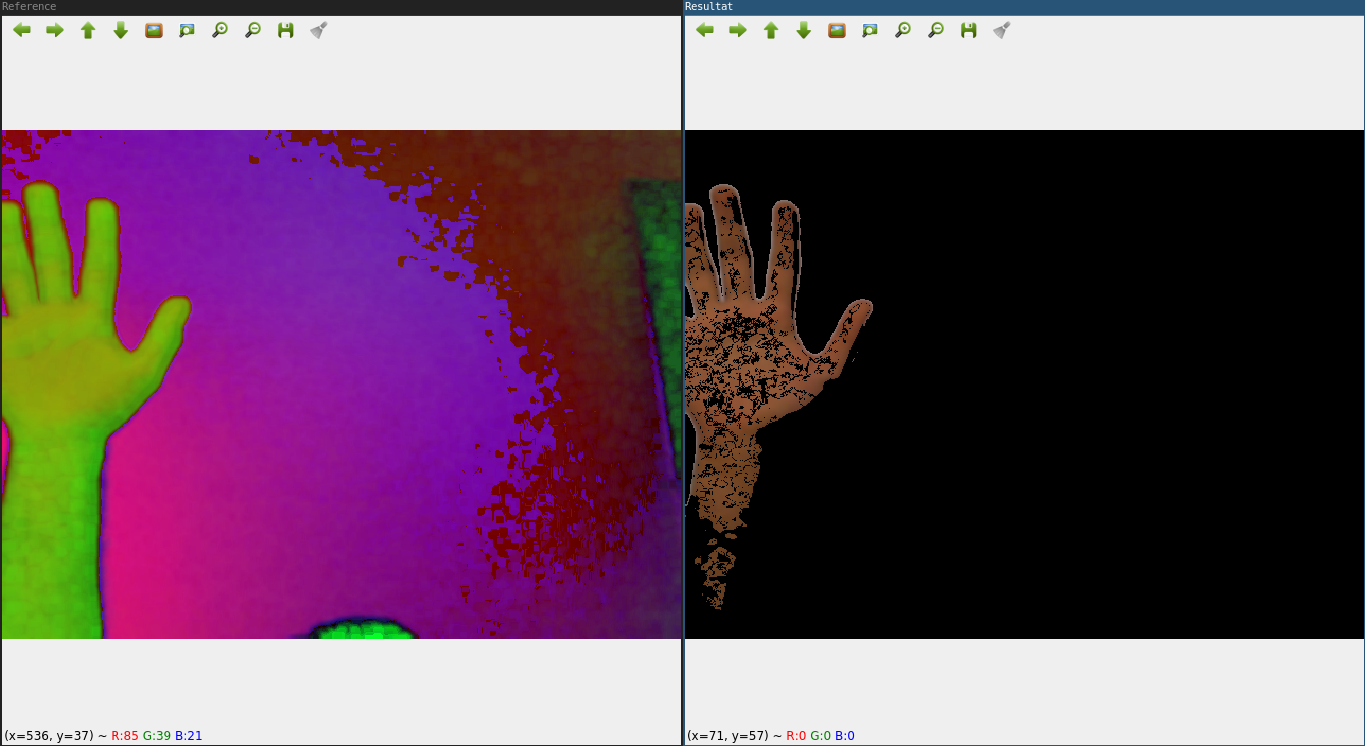
\includegraphics[width=0.8\textwidth]{Images/BGSub/BGSubWithColor.png}\\
        \textit{Suppression du fond et affichage de la couleur original des pixels}
    \end{center}
%%%%%%%%%%%%%%%%%%%%%%%% CAMERA %%%%%%%%%%%%%%%%%%%%%%%%%%%%
\section{Caméra}
\subsection{Calibration}
\subsubsection{Vision}
Lorsque l'on prend une photo, le capteur perçoit un point sur un plan 2D (2 dimension). Le schéma ci-dessous présente un plan orthonormé en 3D, avec comme axes x,y et z. Lorsque l'on inscrit un pixel sur une image, par exemple "m", nous avons pris la valeur du point M sur ses axes x et y car le capteur n'a pas de notion de profondeur, qui est la dimension manquante, la z.

\begin{center}
    \begin{tikzpicture}
    \path(0,-0.2) node{O};
    \path(0,2.2) node{Y};
    \path(2.2,-0.5) node{Z};
    \path(1.5,1.7) node{X};
    \path(8,2.3) node{M(X,Y,Z)};
    \path(3.9,1.3) node{m};
    \path(3.9,0.98) node{x};
    % Repere 0
    \draw[->](0,0) -- (2,-0.5); % Axe Z
    \draw[->](0,0) -- (1.5,1.5); % Axe X
    \draw[->](0,0) -- (0,2); % Axe Y
    % Image perçu
    \draw[-](3,-2)--(3,2); % Gauche
    \draw[-](3,2)--(5,4) ;% Haut
    \draw[-](5,4)--(5,0) ;% Droit
    \draw[-](5,0)--(3,-2); % Bas
    % Exemple de perception d'un point sur une image
    \draw[-](0,0) -- (8,2); % Vecteur M 
    \draw(8,2) circle (0.05); % Vecteur M 
    \end{tikzpicture}
\end{center}

Le point \textbf{M} à pour valeur x,y,z. Que l'on écrit: $$\textbf{M}\begin{bmatrix}x\\y\\z\end{bmatrix}$$

Sur un plan en 2D (Hauteur[Y]/Profondeur[Z]), nous avons:\\

\begin{center}
    \begin{tikzpicture}
    \path(0,-0.2) node{O};
    \path(0,2.2) node{Y};
    \path(6.15,0) node{Z};
    \path(-0.2,0.2) node{X};
    \path(7,1.5) node{M(x,y,z)};
    \path(3.4,0.4) node{V};
    \path(5.7,0.75) node{y};
    \path(1.5,-1) node{f}; % f
    \path(2.75,-2) node{z}; % f
    \path(2.7,1) node{m(u,v)}; % f
    \path(3,0.75) node{x}; % f
    %%%%%%%%%%%%%%%%%%%%%%%%%%%%%%%%%%
    \draw[->](0,0) -- (6,0); % Axe Z
    \draw[->](0,0) -- (0,2); % Axe Y
    \draw[-](0,0) -- (6,1.5); % Vecteur M
    \draw (6,1.5) circle (0.05);
    %%%%%%%%%%%%%%%%%%%%%%%%%%%%%%%%%%%
    \draw[-,dashed](3,-1) -- (3,2); % Barre V
    \draw[-,dashed](5.5,-2) -- (5.5,2); % Barre Y
    \draw[<->](0,-0.65) -- (3,-0.65); % Barre f 
    \draw[<->](0,-1.5) -- (5.5,-1.5); % Barre z
    \end{tikzpicture}
\end{center}
Ce point de vue nous permet d'appliquer le théorème de Thalès pour récupérer des informations. Nous pouvons effectuer : $\frac{v}{y}$ = $\frac{f}{z}$ \\

Ainsi on peut en déduire de : $v=\frac{fY}{z}$ et $u=\frac{fX}{Z}$

\subsubsection{Erreur de centrage}

Nous pouvons écrire la matrice: 
$$\left\{ 
    \begin{array}{ll}
        v=\frac{fY}{Z}+V0  \\ \\
        u=\frac{fX}{Z}+U0
    \end{array} \\
\right. $$ \\

Que l'on peut écrire: 
$$\left\{ 
    \begin{array}{ll}
        v=\frac{fY+V0Z}{Z} \\ \\
        u=\frac{fX+U0Z}{Z}
    \end{array} \\
\right. $$

La préférence de coordonnée homogène nous fait écrire le système:
$$\left\{ 
    \begin{array}{ll}
        v'=fY+U0\\ \\
        u'=fX+U0 \\ \\
        w'=Z
    \end{array} \\
\right. $$

Avec ces nouvelles forme d'écriture nous écrivons: $u=\frac{u'}{w'}$ et $v=\frac{v'}{w'}$

\subsubsection{Matrice de projection}
Ainsi la matrice s'écrit:
$$\begin{matrix}
    
    \underbrace{\begin{bmatrix}
        u'\\v'\\w'\\
    \end{bmatrix}}_{\text{Coord. H. pixel}}
    
    =\hspace{0.2cm}
    
    \underbrace{\begin{bmatrix}
        \alpha f & \textit{s} & u0\\
        0 & \beta f & v0\\
        0 & 0 & 1\\
    \end{bmatrix}}_{\text{Matrice de projection}}
    
    \hspace{0.5cm}
    
    \underbrace{\begin{bmatrix}
        X\\Y\\Z\\
    \end{bmatrix}}_{\text{Coord. 3D du point}}
\end{matrix}$$

\textit{ \textbf{$\alpha$} et \textbf{$\beta$} sont la densité de pixel et \textbf{s} est le "skew"(qui tant vers 0).}\\

Si nous avons la valeur de \textbf{u} et de \textbf{v}, par exemple: u=310, v=240, nous avons pas le moyen de savoir la valeur de \textbf{w} (étant le facteur de profondeur de l'objet).\\
Il faut passer sous un modèle 3D:

\begin{center}
    \begin{tikzpicture}
        \path(6,-2.2) node{O\tiny{1}};
        \path(0,-0.2) node{O\tiny{0}};
        \path(3,1.2) node{\textbf{w}};
        \path(4,1.55) node{\textbf{w1}};
        \path(5,1.85) node{\textbf{w2}};
        \path(6,2.15) node{\textbf{w3}};
        \path(0,-0.2) node{O\tiny{1}};
        
        % Repere 
        \draw[->](0,0) -- (0,2); 
        \draw[->](0,0) -- (3.5,0); 
        \draw[->](6,-2) -- (4.5,-1); 
        \draw[->](6,-2) -- (6.5,-1); 
        
        % Exemple de perception d'un point sur une image
        \draw[-](0,0) -- (6,2);
        \draw[-](6,-2) -- (2.5,1.5);
        \draw(3,0.99) circle (0.05);
        \draw(4,1.33) circle (0.05);
        \draw(5,1.66) circle (0.05);
        \draw(6,1.99) circle (0.05);
    \end{tikzpicture}
\end{center}
 
Avoir une deuxième point de vue nous permet de définir \textbf{w}.
 
 \subsubsection{Changement de repères}
 
 \begin{center}
    \begin{tikzpicture}
        \path(0,-0.2) node{R\tiny{0}};
        \path(3,-2.2) node{R\tiny{1}};
        \path(5,1) node{x};
        \path(6,1) node{\textbf{M$\begin{pmatrix}x\\y\\z\end{pmatrix}$}};
        \path(6.7,0.3) node{R\tiny{0}};
        % Repères
        \draw[->](0,0) -- (0,2); 
        \draw[->](0,0) -- (2,0);
        \draw[->](3,-2) -- (3,0); 
        \draw[->](3,-2) -- (5,-2);
        % Marqueur
        \draw(5,1) circle (0.18);
        % Visu CAM
        \draw[->](0,0) -- (3,0.65);
        \draw[->](3,-2) -- (4.35,0);
        % Arc de cercle
        \draw[<->] (2,-2) arc (-85:-170:1.7);
     \end{tikzpicture}
\end{center}

Pour passer de la vue R\small{0} à la vue R\small{1} il faut utiliser une matrice de passage:\\

$$ \begin{matrix}
    
    \begin{pmatrix}
        x\\y\\z\\1
    \end{pmatrix}_{\text{R1}}
    
    =
    
    \underbrace{^1T_^0}_{\text{Matrice de passage R0 vers R1}}
    
    \hspace{0.5cm}
    
    \underbrace{\begin{pmatrix}
        X\\Y\\Z\\1\\
    \end{pmatrix}_{\text{R0}}}_{Sur le plan 0}
    
\end{matrix}$$\\

La matrice de passage donne:


$$ \begin{matrix}
    
    \begin{pmatrix}
        x\\y\\z\\1
    \end{pmatrix}_{\text{R1}}
    =
    \underbrace{\begin{pmatrix}
    R_^1^1 & R_^1^2 & R_^1^3 & T_^x  \\
    R_^2^1 & R_^2^2 & R_^2^3 & T_^y  \\
    R_^3^1 & R_^3^2 & R_^3^3 & T_^z  \\
    0 & 0 & 0 & 1 \\
    \end{pmatrix}}_{\text{Matrice de passage R0 vers R1}}
    \hspace{0.5cm}
    \begin{pmatrix}
        X\\Y\\Z\\1\\
    \end{pmatrix}_{\text{R0}}
    
\end{matrix}$$

Où: 
    \begin{center}
    \begin{matrix}
        R_^1^1 & R_^1^2 & R_^1^3   \\
        R_^2^1 & R_^2^2 & R_^2^3  \\
        R_^3^1 & R_^3^2 & R_^3^3   
    \end{matrix}
    \end{center}
Est la matrice de rotation. Et: \\
    \begin{center}
    \begin{matrix}
         T_^x  \\
         T_^y  \\
         T_^z  
    \end{matrix}
    \end{center}
Est la matrice de translation.

\subsubsection{Vision stéréo}
Le principe de la Vision stéréo est de pouvoir retrouver la position d'un objet sur un espace 3D via plusieurs vues de lui même.
 \begin{center}
    \begin{tikzpicture}
        \path(0,-0.7) node{Caméra0};
        \path(0,-0.2) node{X};
        \path(0,2.3) node{Y};
        \path(2.2,0) node{Z};
        \path(0,-4.2) node{Caméra1};
        \path(6,0.5) node{x};
        \path(7,0.5) node{\textbf{M\begin{pmatrix}X\\Y\\Z\end{pmatrix}}};
        \path(3.5,0.6) node{u,v};
        \path(3.5,-2) node{u',v'};
        % Marqueur
        \draw(6,0.5) circle (0.18);
        \draw(3,0.25) circle (0.05);
        \draw(3,-1.75) circle (0.05);
        % Plan
        \draw[-](3,0) -- (3,2); 
        \draw[-](3,-4) -- (3,-1); 
        % Repères
        \draw[->](0,0) -- (0,2); 
        \draw[->](0,0) -- (2,0);
        \draw[->](0,-4) -- (0,-2); 
        \draw[->](0,-4) -- (2,-4);
        % Visu CAM
        \draw[-](0,0) -- (6,0.5);
        \draw[-](0,-4) -- (6,0.5);
     \end{tikzpicture}
\end{center}

On peu en déduire que: \\

Camera 0: $$\begin{bmatrix}U\\V\\W\\ \end{bmatrix} 
=
\begin{bmatrix}
    f & 0 & u0\\
    0 & f & v0\\
    0 & 0 & 1\\
\end{bmatrix}
\begin{bmatrix}
    X\\Y\\Z
\end{bmatrix}_{\text{\tiny{0}}}$$

Camera 1: $$\begin{bmatrix}U'\\V'\\W'\\ \end{bmatrix}
=
\begin{bmatrix}
    f' & 0 & u0'\\
    0 & f' & v0'\\
    0 & 0 & 1\\
\end{bmatrix}
\begin{bmatrix}
    X\\Y\\Z
\end{bmatrix}_{\text{\tiny{1}}}$$\\
On va définir Caméra 1 sur le plan 0.

$$\text{Camera 1=}\begin{bmatrix}
    f' & 0 & u0'\\
    0 & f' & v0'\\
    0 & 0 & 1\\
\end{bmatrix}
\begin{bmatrix}
    ^1T_^0
\end{bmatrix}
\begin{bmatrix}
    X\\Y\\Z\\
\end{bmatrix}_{\text{\tiny{0}}}
=
\begin{bmatrix}
    f' & 0 & u0'\\
    0 & f' & v0'\\
    0 & 0 & 1\\
\end{bmatrix}
\begin{bmatrix}
    R_^1^1 & R_^1^2 & R_^1^3 & T_^x  \\
    R_^2^1 & R_^2^2 & R_^2^3 & T_^y  \\
    R_^3^1 & R_^3^2 & R_^3^3 & T_^z  \\
    0 & 0 & 0 & 1 \\
\end{bmatrix}
\begin{bmatrix}
    X\\Y\\Z\\
\end{bmatrix}_{\text{\tiny{0}}}
$$

\subsubsection{Géométrie épipôlaire}

La géométrie épipôlaire permet d'établir une relation géométrique entre deux images d'une même scène.\\

 \begin{center}
    \begin{tikzpicture}
        % Visu CAM
            \draw[-](0,0) -- (1.5,1.5); % /
            \draw[-](0,0) -- (2,0); % _
            \draw[-](8,0) -- (6.5,1.5); % \
            \draw[-](8,0) -- (6,0); % _
        % Path
            \path(0,-0.2) node{Cam0};
            \path(8,-0.2) node{Cam1};
            \path(-0.5,2) node{Plan0};
            \path(8.5,2) node{Plan1};
            \path(4,4.5) node{Point};\draw(4,4) circle (0.1);
            \path(1.4,0.7) node{E0}; % Epipole 0
            \path(6.6,0.7) node{E1}; % Epipole 1
            \path(1.3,1.5) node{p};  
            \path(1.8,-0.2) node{e};  
            \path(6.8,1.6) node{p'};
            \path(6.2,-0.2) node{e'};  
        % Plan 0
            \draw[-](2,-1) -- (2,2); % plan0 | Droit
            \draw[-](2,-1) -- (0,1); % plan0 \ Bas
            \draw[-](0,1) -- (0,4); % plan0 | Gauche
            \draw[-](0,4) -- (2,2); % plan0 \ Haut
        %%%%%%%%%%%%%%%%%%%%%%%%%%%%%%%%%%%%%%
            \draw[-,densely dotted](2.1,0) -- (5.9,0); % plan0
        %%%%%%%%%%%%%%%%%%%%%%%%%%%%%%%%%%%%%%
        % Plan 1
            \draw[-](6,-1) -- (6,2); % plan1 | Gauche 
            \draw[-](8,4) -- (6,2); % plan0 / Bas
            \draw[-](8,1) -- (8,4); % plan0 | Droit
            \draw[-](6,-1) -- (8,1); % plan0 / Haut
        % Point to Cam 
            \draw[-,densely dotted](4,4) -- (2,2); % Point to cam0
            \draw[-,densely dotted](4,4) -- (6,2); % Point to cam1
        % Droites épipolaires
             \draw[-,dashed](1.5,1.5) -- (1.9,0); % Plan 0
             \draw[-,dashed](6.1,0) -- (6.5,1.5); % Plan 1
        % Marqueur
            \draw(1.9,0) circle (0.05); % Plan 0 B
            \draw(1.5,1.5) circle (0.05); % Plan 0 H
            \draw(6.5,1.5) circle (0.05); % Plan 1 B
            \draw(6.1,0) circle (0.05); %Plan 1 H
     \end{tikzpicture}
\end{center}

% URL https://slideplayer.fr/slide/1304090/
\begin{itemize}
    \item[$\bullet$] Un épipôle est le centre de projection d'une caméra vue dans le plan image de l'autre caméra. Seul une droite épipolaire passe par chaque point des images (sauf aux épipôles)
    \item[$\bullet$] Une droite épipolaire est formé par l'épipôle et une point de l'image (multitude de droites épipôlaires par image)
\end{itemize}

Donc: \\
\begin{itemize}
    \item \textbf{E0} et \textbf{E1} sont les droites épipôlaires
    \item \textbf{e} et \textbf{e'} sont les épipôles gauche et droit
    \item \textbf{e} est l'origine de \textbf{Cam1} vue de \textbf{Cam0} et \textbf{e'} est l'origine de \textbf{Cam0} vue de \textbf{Cam1}
\end{itemize} 

\subsubsection{Calibrage d'une caméra}

En tenant compte des dimensions du pixel nous avons 2 facteur qui s'insèrent dans la matrice: \textbf{$\alpha$} et \textbf{$\beta$}.\\

\begin{center}
    $\begin{matrix}
        \begin{bmatrix}
            u\\v\\w\\
        \end{bmatrix}
        =
        \begin{bmatrix}
            \alpha fx &0 &Uo\\
            0&\beta fy&Vo\\
            0&0&1
        \end{bmatrix}
        \begin{bmatrix}
            X\\Y\\Z\\
        \end{bmatrix}
    \end{matrix}$
\end{center}\\
\begin{itemize}
    \item Avec notre capteur, \textbf{$\alpha$} et \textbf{$\beta$} ont pour valeur:  $\frac{1}{25}$ pixel/$\mu$m.
    \item \textbf{x} et \textbf{y} sont exprimés en mètre.
    \item \textbf{$\alpha$ fx} et \textbf{$\beta$ fy} sont alors exprimés en pixel.mètre . 
    \item Uo et Vo  sont exprimés en pixel. 
\end{itemize}







\end{document}



% Ligne de codes
\begin{minted}[
    baselinestretch=1.4,
    bgcolor=lightgray,
    fontsize=\footnotesize]
{c++}

\end{minted}



\begin{center}
    \begin{tikzpicture}
  
        \path(3.5,-2) node{u',v'};
        % Marqueur
        \draw(3,-1.75) circle (0.05);
        % Plan
        \draw[-](3,-4) -- (3,-1); 
        % Repères
        \draw[->](0,0) -- (0,2); 
        % Visu CAM
        \draw[-](0,0) -- (6,0.5);
     \end{tikzpicture}
\end{center}

$$\begin{matrix}
    
    \underbrace{\begin{bmatrix}
        u'\\
    \end{bmatrix}}_{\text{Coord. H. pixel}}
    =
    \underbrace{\begin{bmatrix}
        \alpha f \\
    \end{bmatrix}}_{\text{Matrice de projection}}
    \underbrace{\begin{bmatrix}
        X\\
    \end{bmatrix}}_{\text{Coord. 3D du point}}
\end{matrix}$$
